%  DEFRAG Presentation
%
% 12 Novebmer 2012
% Scott Hendrickson
% @DrSkippy27
% Gnip Inc
% 

\documentclass{beamer}
\setbeamertemplate{navigation symbols}{}

% THEMES
%\usetheme{Bergen}
%\usetheme{Singapore}
\usetheme{gnip}

\usepackage[group-separator={,}]{siunitx}
%\usepackage{fontspec}
\setbeamertemplate{footline}[text line]{
    \colorbox{white}{\parbox[22px]{\paperwidth} {\color{linecolour} {\line(1,0){500} \\ \hfill Gnip Inc.   @DrSkippy27}}}
}

\beamersetuncovermixins{\opaqueness<1>{25}}{\opaqueness<2->{15}}

\usepackage{minted}
\usepackage{tikz}

\begin{document}
\title{Social media pulse: The shape of breaking news on social media}  
\author{Scott Hendrickson \\ Data Scientist  \\ Gnip Inc.\\ @DrSkippy27}
\date{\today} 

% title

\begin{frame}
\titlepage
\end{frame}

% staging the question

\begin{frame}
\begin{center}
{\Huge why social media for breaking stories? }
\end{center}
\end{frame}

% "accelerating the aha moment"

\begin{frame}
\begin{center}
{\Huge 1. audience, perspective and coverage }
\end{center}
\end{frame}

\begin{frame}
\begin{center}
{\Huge 2. speed }
\end{center}
\end{frame}

\begin{frame}
\begin{center}
{\Huge 3. richness, diversity }
\end{center}
\end{frame}

%%  audience, perspective and coverage

\begin{frame}
\begin{center}
{\Huge many publishers: audience, perspective and coverage }
\end{center}
\end{frame}

% volumes
%wporgcom 760k
%wporg 300k
%wpcomcom 260k
%wpcom 315k
%idebate 108k
%wp likes 181k
%disqus com 1.28M
%disqus votes 2.25M
%disqus post votes 109k

\begin{frame} 
\begin{table}
\begin{tabular}{l|r}
\hline
   {Publisher}   &   {Daily Activity}   \\
\hline 
    Twitter      &      400M   \\
    Tumblr      &        75M   \\
    Wordpress Posts &     615k   \\
    Wordpress Comments & 1.1M \\
    Disqus       &       1.3M  \\
    Engagement (likes, votes) & 2.4M  \\
\hline
\end{tabular}
\end{table}
\end{frame}

% flooding

\begin{frame}
  \begin{center}
    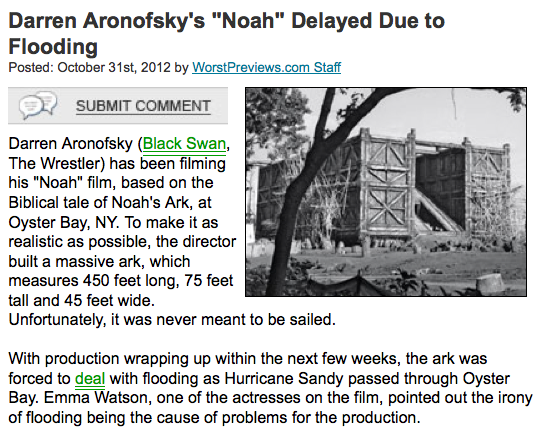
\includegraphics[width=7cm]{./imgs/flooding.png}
  \end{center}
\end{frame}

% signal vs. noise

\begin{frame}
\begin{center}
\center{\Huge {noise or signal?}}
\end{center}
\end{frame}

% chelsea con-ed example

\begin{frame}
  \begin{center}
    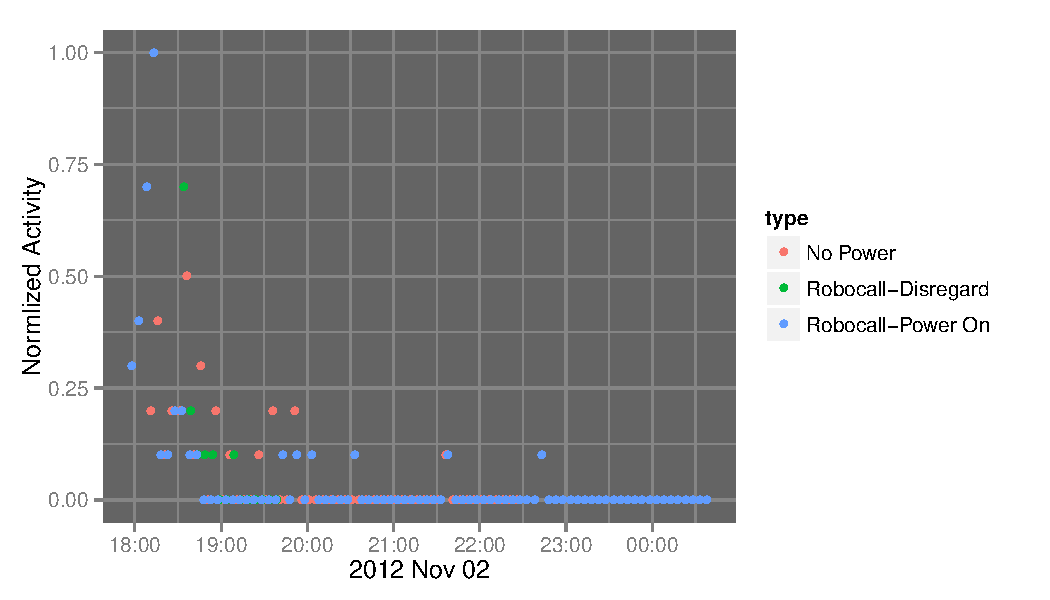
\includegraphics[width=8cm]{./imgs/fake.pdf}
  \end{center}
\end{frame}

\begin{frame}
  \begin{center}
    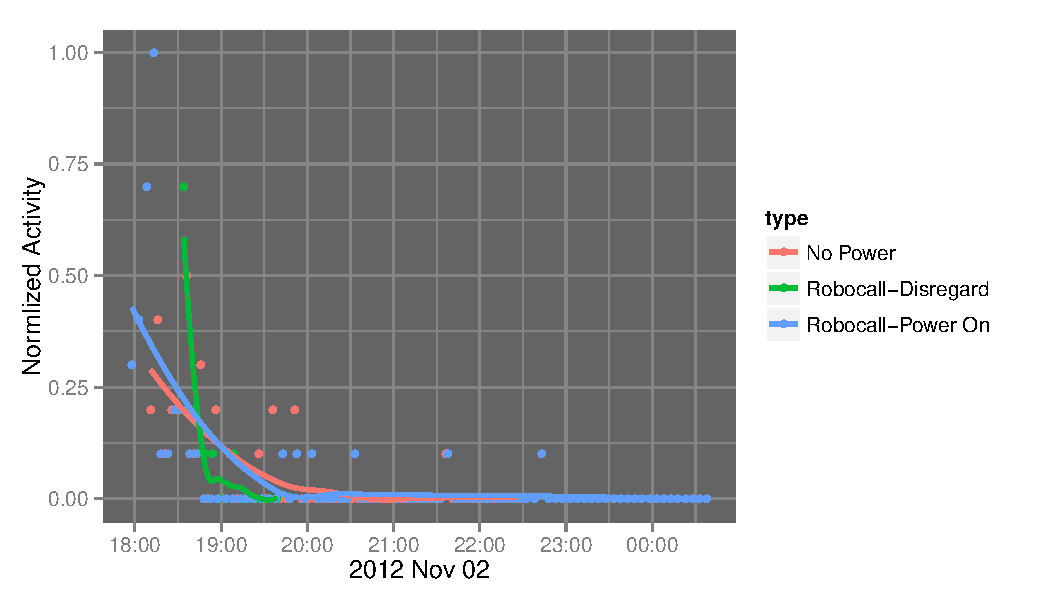
\includegraphics[width=8cm]{./imgs/fake_fit.pdf}
  \end{center}
\end{frame}

\begin{frame}
  \begin{center}
    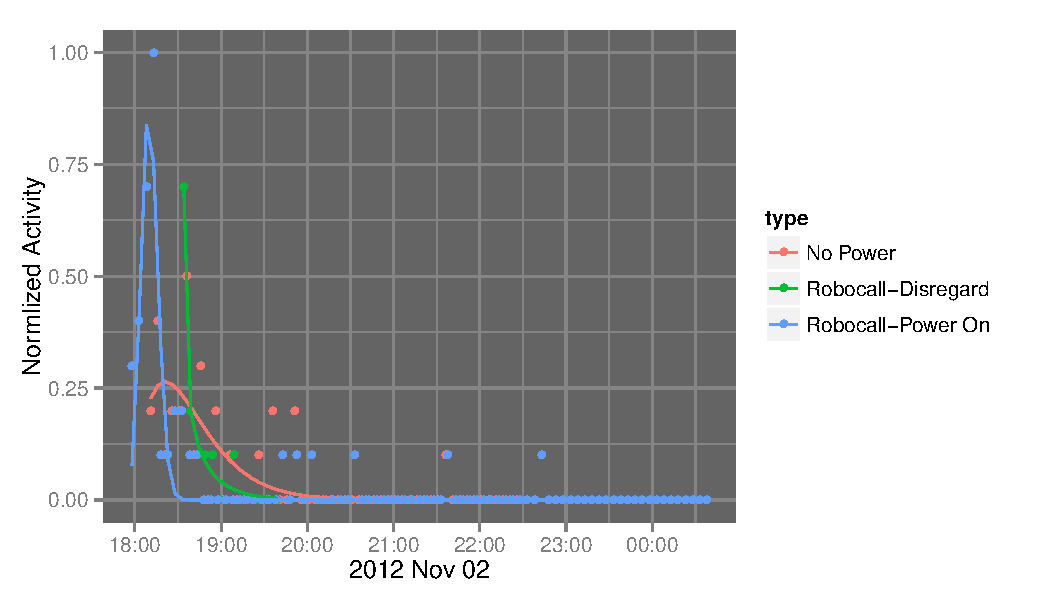
\includegraphics[width=8cm]{./imgs/fake_fit2.pdf}
  \end{center}
\end{frame}

\begin{frame}
  \begin{center}
    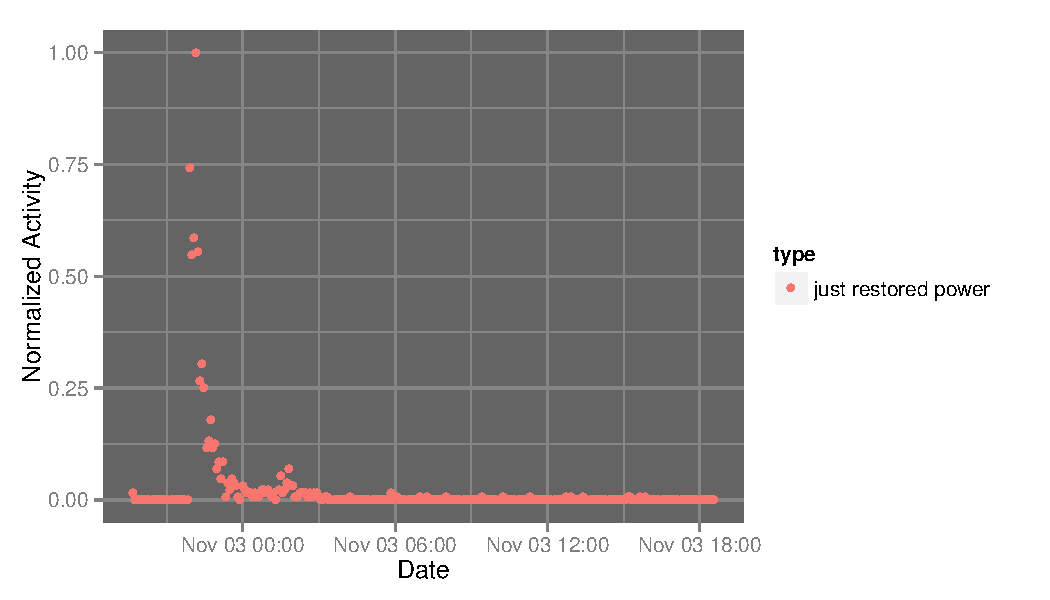
\includegraphics[width=8cm]{./imgs/real.pdf}
  \end{center}
\end{frame}

\begin{frame}
  \begin{center}
    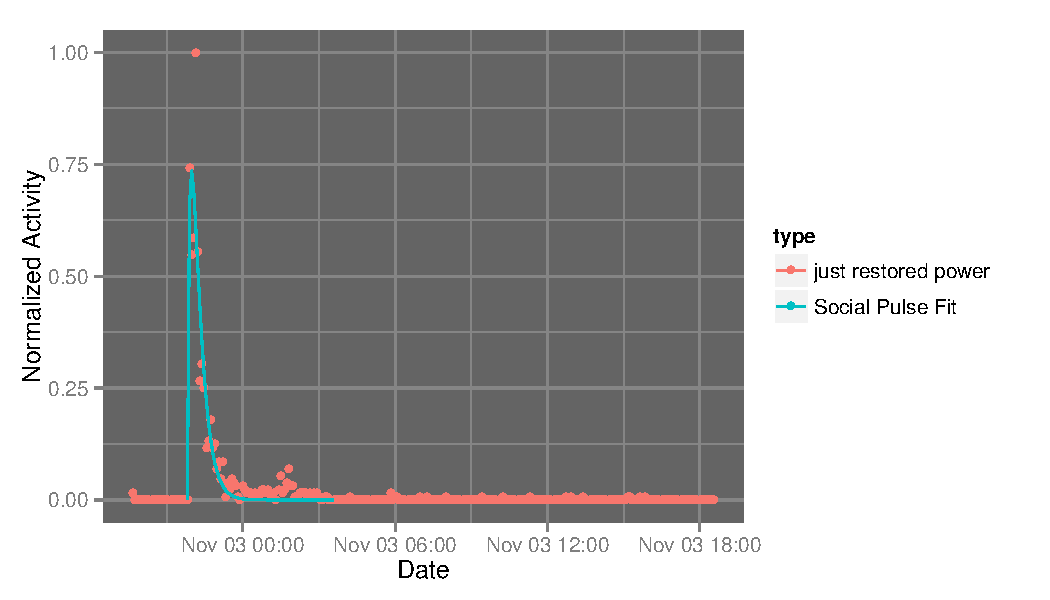
\includegraphics[width=8cm]{./imgs/real_fit.pdf}
  \end{center}
\end{frame}

% speed

\begin{frame}
\begin{center}
{\Huge realtime firehose: speed}
\end{center}
\end{frame}

% Events

\begin{frame}\frametitle{Events}
\begin{table}
\begin{tabular}{ m{2cm} | m{ 2.5cm} | m{4cm}}
\hline
Type & Response & Examples \\ \hline
Expected    & Approx. \newline Symmetric & Hurricane Sandy \newline Olympics \\ \hline
Unexpected (many obs.) & Social Media \newline Pulse & Beyonce' VMAs \newline  Mexico earthquake \newline  Steve Jobs \\ \hline
Unexpected (spread) & Sigmoid \newline Pulse & Osama Bin Laden \newline  Whitney Houston \newline  Syrian dissidents \\ \hline
\end{tabular}
\end{table}
\end{frame}

% half life

\begin{frame}\frametitle{Half-life}
\begin{center}
{\Huge time to observe \\[6pt] $\frac{1}{2}$ of the activities \\[6pt] for an event}
\end{center}
\end{frame}

\begin{frame}
\frametitle{Social media pulse} 
Given an event, the probability of a activity from one person,

\begin{equation*}
f(t) = \lambda \exp(-\lambda t), \text{ for } t \geq 0.
\end{equation*}

Many people posting, so sum of random variables $S = X_1 + X_2 + \ldots + X_{n \text{ posters}}$.

Probability distribution function,

\begin{equation*}
f_S(t) = \frac{ \beta^{-\alpha} t^{\alpha-1} \exp( \frac{-t}{\beta}) } {\Gamma(\alpha)}
\end{equation*}

Cumulative distribution is the ``generalized regularized incomplete gamma function'',

\begin{equation*}
F_S(t) = Q(\alpha, 0, \frac{ t}{\beta})
\end{equation*}
\end{frame}

% gamma plots

\begin{frame}
  \begin{center}
   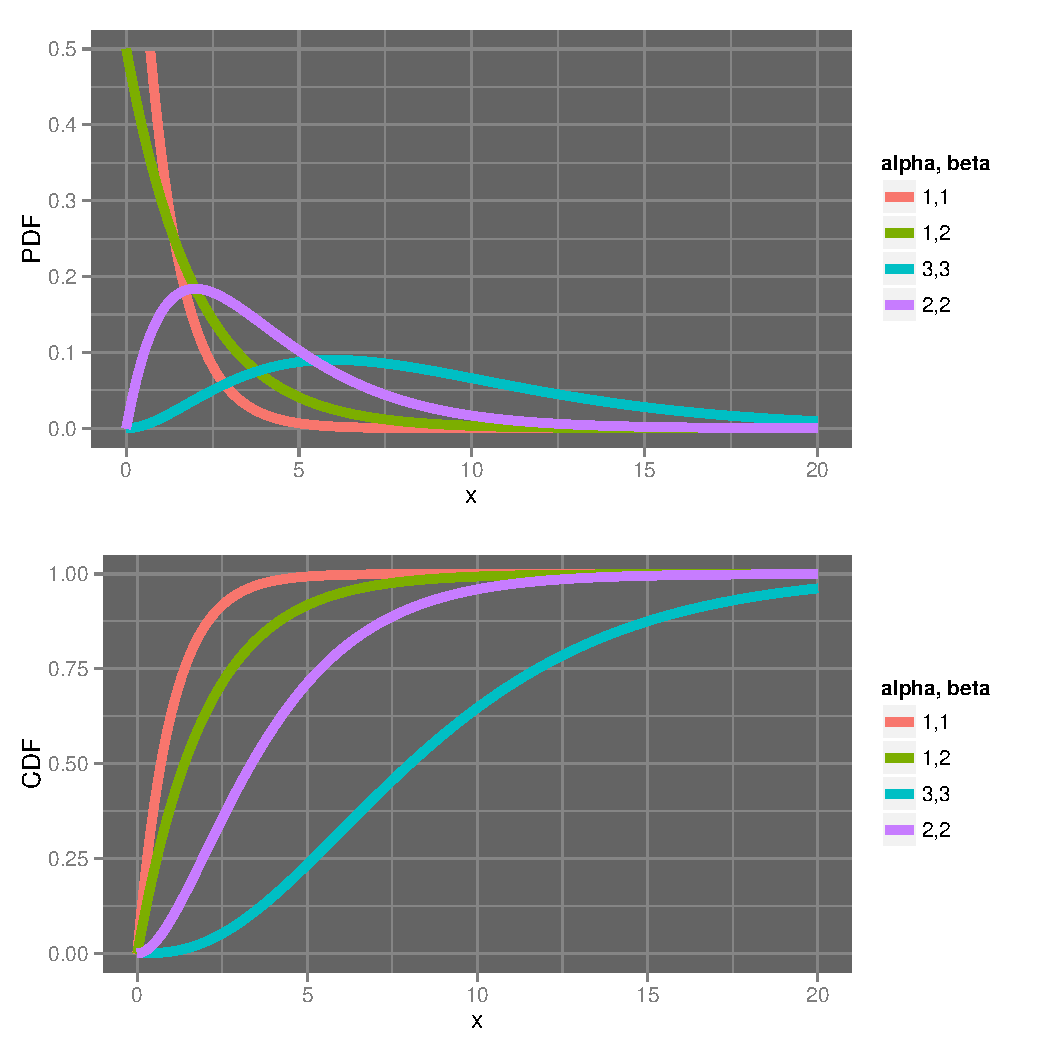
\includegraphics[height=6cm]{./imgs/gammadist.pdf}
  \end{center}
\end{frame}

\begin{frame} \frametitle{Publishers}
\begin{table}
\begin{tabular}{l|c}
\hline
   {Publisher}   &   {Speed} \\
\hline 
    Twitter      &    Fast  \\ 
    Tumblr      &        Fast and Slow \\
    Wordpress Posts &   Fast and Medium   \\
    Wordpress Comments & Fast\\
    Disqus       &    Fast\\
    Engagement (likes, votes) &  Fast\\
\hline
\end{tabular}
\end{table}
\end{frame}

% JPMorgan

\begin{frame}
  \begin{center}
    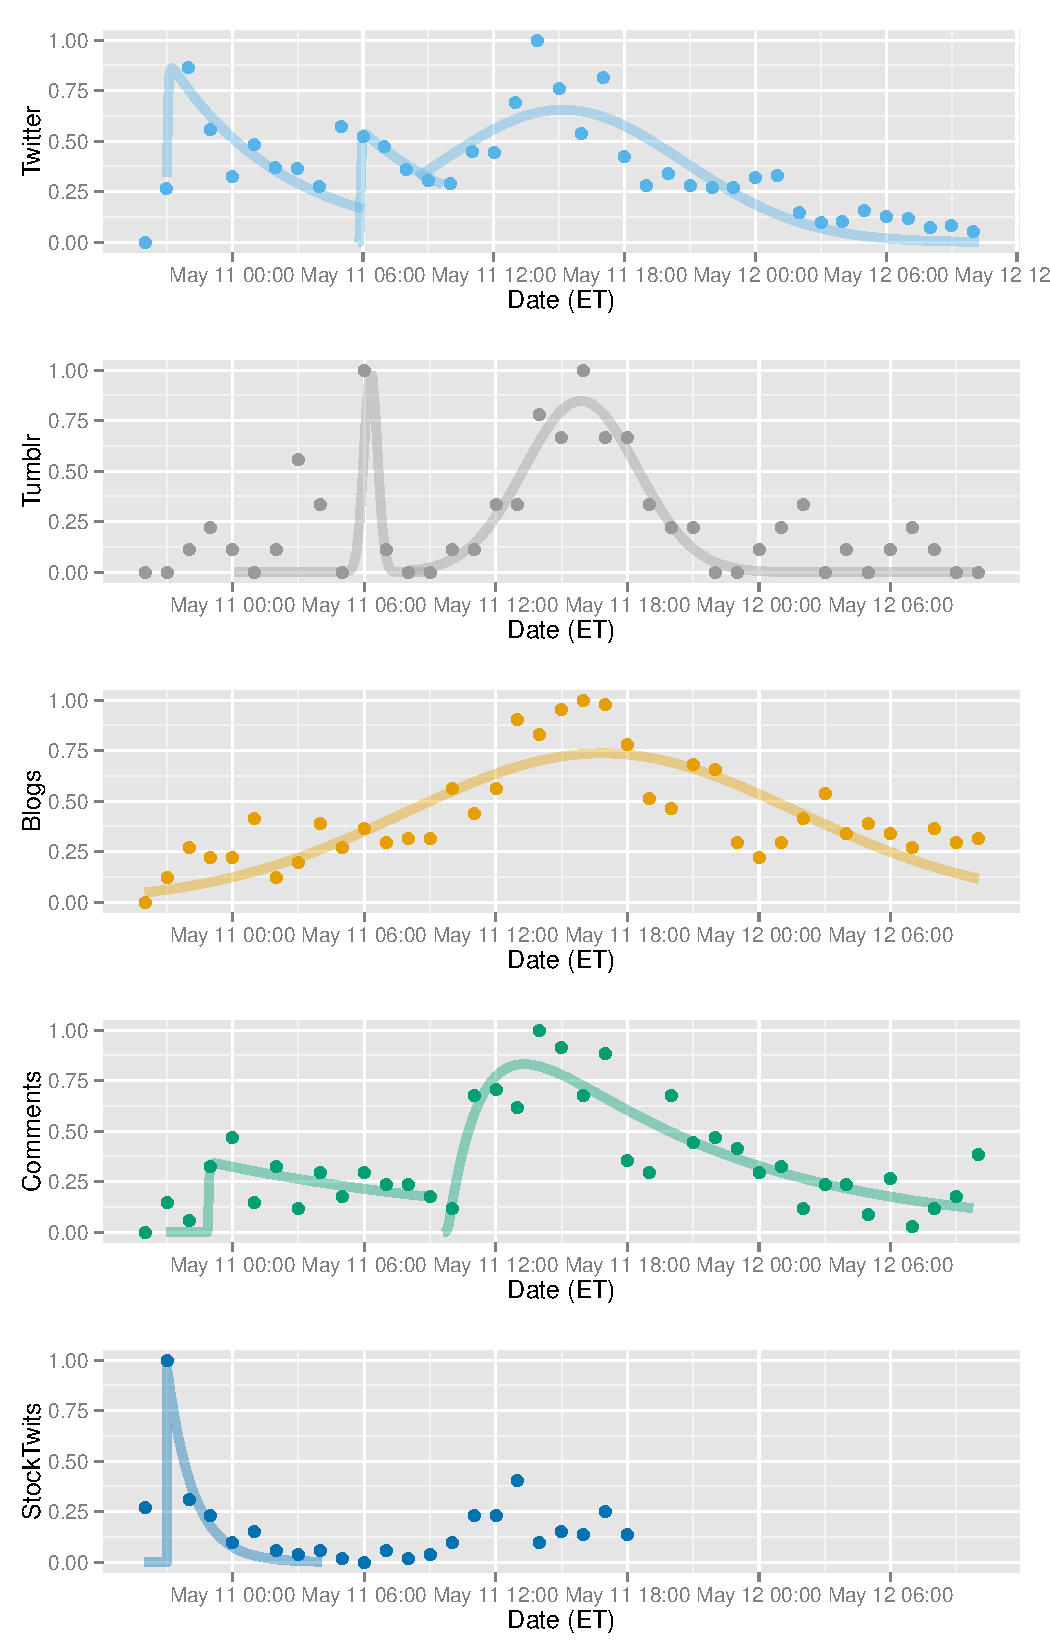
\includegraphics[height=8.5cm]{./imgs/JPMorgan.pdf}
  \end{center}
\end{frame}


%%  richness

\begin{frame} \frametitle{Speed and Richness}
\begin{table}
\begin{tabular}{m{2cm}| c |m{3cm}}
\hline
   {Publisher}   &   {Speed} & {Richness} \\
\hline 
    Twitter       & Fast & Concise  \\ [3pt]
    Tumblr       & Fast, Slow & Rich, multimedia\\  [3pt]
    Wordpress Posts & Fast, Medium &  Rich, text\\  [3pt]
    Wordpress Comments  & Fast & Reactive, small-to-medium\\  [3pt]
    Disqus         & Fast & Reactive, small-to-medium\\  [3pt]
    Engagement   & Fast & Terse\\ 
\hline
\end{tabular}
\end{table}
\end{frame}

% summary speed and richness

\begin{frame}\frametitle{Social Cocktail}
  \begin{center}
    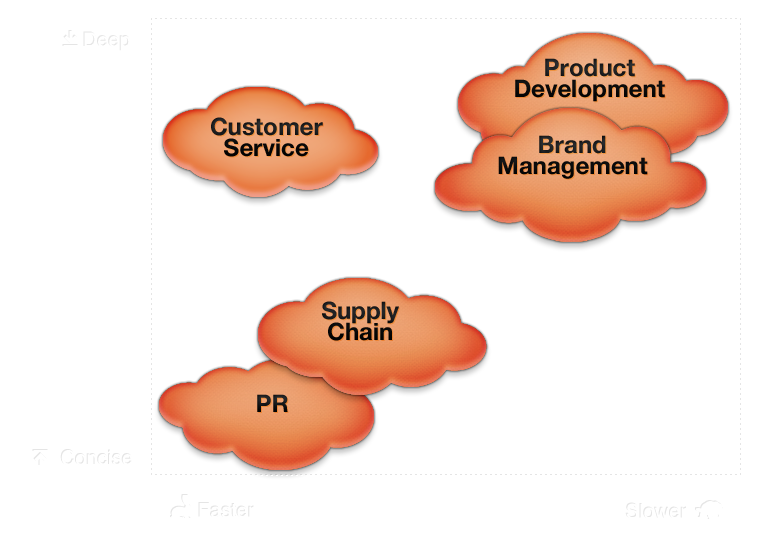
\includegraphics[width=7cm]{./imgs/socialcocktailgrid.png}
  \end{center}
\end{frame}

% sink fail

\begin{frame}\frametitle{Without Gnip\ldots}
  \begin{center}
    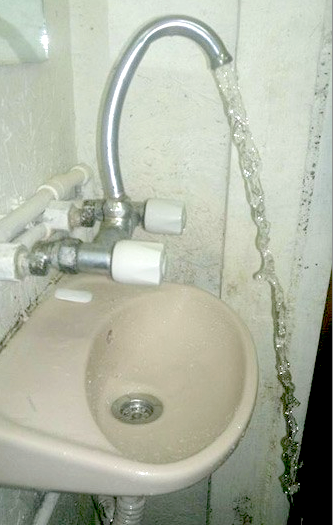
\includegraphics[width=4cm]{./imgs/sinkfail.png}
  \end{center}
\end{frame}


%
\begin{frame}
\begin{center}
{\Huge Filter: match terms (AND, OR, NOT), metadata }
\end{center}
\end{frame}


\begin{frame}
\begin{center}
{\Huge Shape: sample, redundancy, replay }
\end{center}
\end{frame}


\begin{frame}
  \begin{center}
  \Large{Thank you!  \\ [20pt]}
    
\includegraphics[width=3cm]{./imgs/logo.png} \\ [15pt]
   \Large{Presentation, data, code at: github.com/DrSkippy27/Defrag2012 }
  \end{center}
\end{frame}

\end{document}
